\chapter{Implementation}


%5\section{Extension Structure}

As explained in \ref{browserExtensions}, the extension is split into different files for both security reasons and other separation of concerns.
The diagram below puts into more detail the exact structure of the extension in context with some of the real files being used.


\begin{figure}[h]
	\centering
	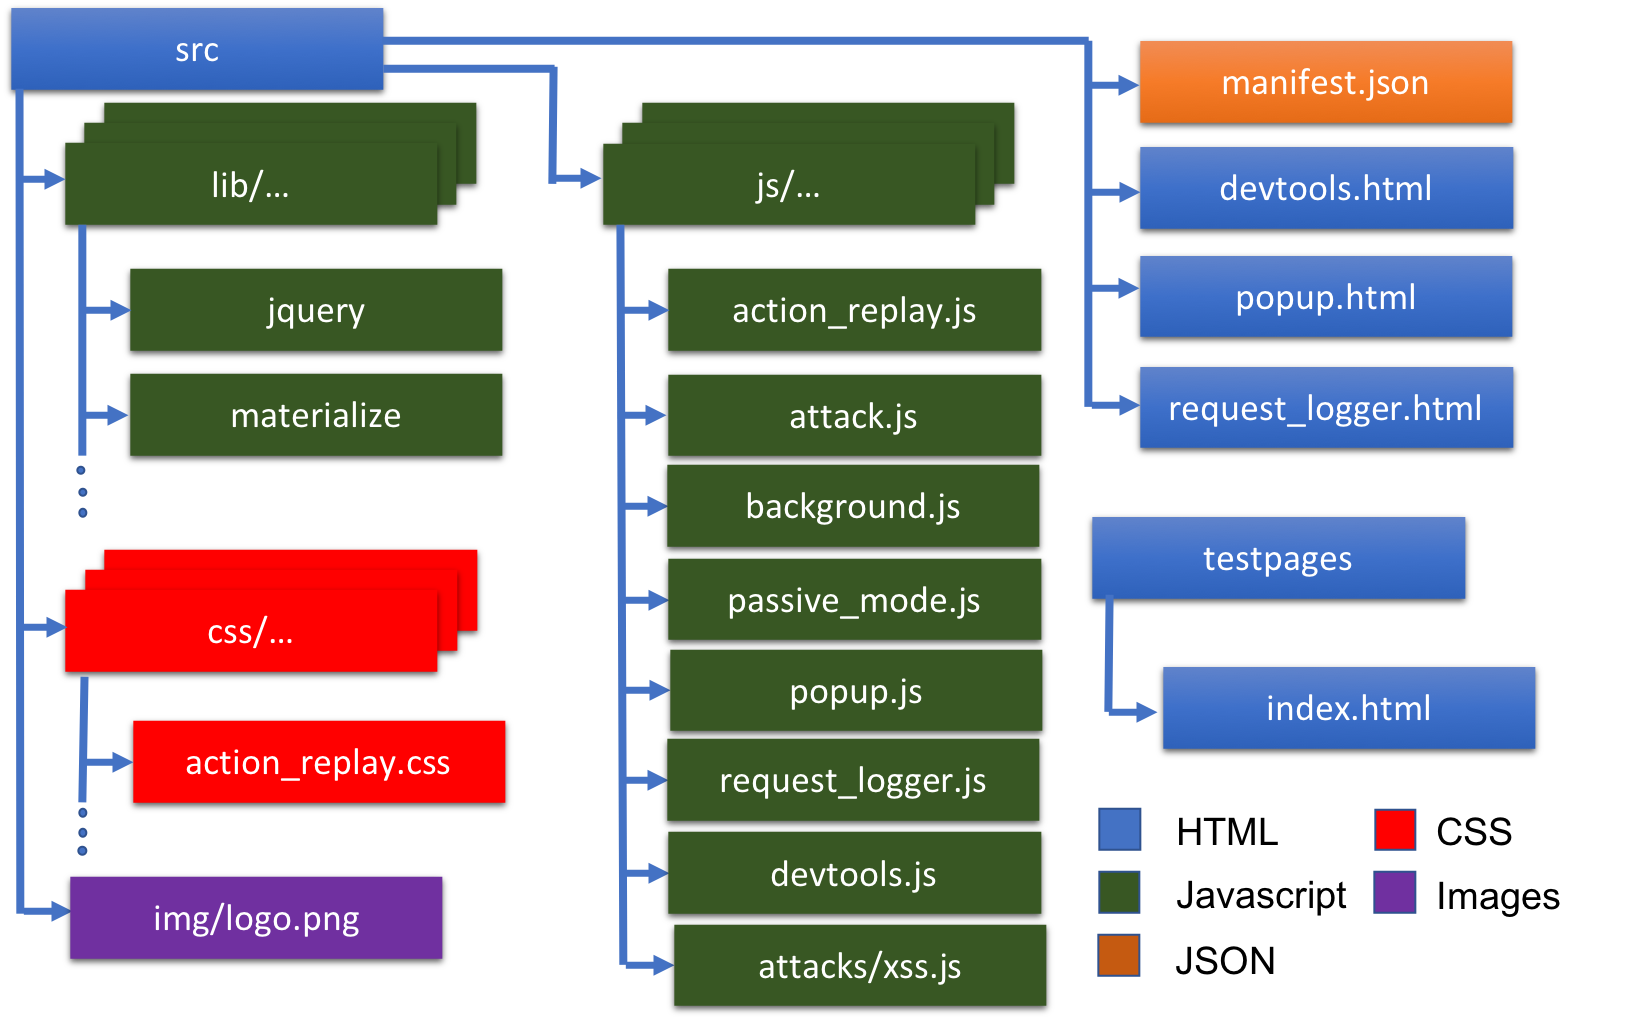
\includegraphics[width=0.9\textwidth]{images/project_structure.png}
	\caption{The directory structure used for the project}
	\label{fig:test}
\end{figure}

I have arranged the files in question into 2 separate subfolders - the \texttt{testpages} directory keeps the source code for the test harness page with vulnerabilities, while the \texttt{src} directory keeps all the other extension related code. \\

Within \texttt{src} we find different folders for separate concerns - \texttt{lib} stores any library code I have imported from a third-party, \texttt{css} keeps custom styles used across the extension, \texttt{img} is where any images are kept, \texttt{js} holds any custom produced Javascript files, and is where most of the logic within the extension lives. \texttt{src} also contains the \textit{manifest} file, and any HTML page code. 

\section{Manifest}

The manifest is where the extension declares its intentions by enumerating all the scripts and files to be accessed, as well as the permissions required to run the extension as an add-on to the browser. This file is necessary due to security reasons; each extension is expected to run as a standalone program within the browser. Any dependencies are to be declared and included within the package before the program is run, with the exception of contents that are whitelisted in the declared \textit{Content Security Policy} (CSP) directive within the file. I am using the recommended default CSP directive of \texttt{script-src 'self'; object-src 'self'}. This policy actively prevents notoriously dangerous Javascript functions from being evaluated, disables in-line Javascript functionality (which enforces a separation of content from behaviour), and, as the name suggests, will only load scripts and files locally available to the package \cite{chromeExtensionCSP}. \\ 

A potential methodology to use in a setting like this would be to employ a bundler to create a single minified (or compressed) \texttt{.js} file that includes all the required libraries and code to be imported. An example of this is  \textit{Webpack} \footnote{\url{https://webpack.js.org/}} - I did not employ a bundler like this as I learned about its uses later into the project. Furthermore, I am including a relatively small number of third-party sourced code, making this a small practical concern. \\

Other noteworthy details from the manifest file include:

\begin{itemize}
	\item The \texttt{devtools\_page} directive - this is necessary to access the developer tools API's within the extension, which provide extra information when using the extension such as the contents of the requests sent at any given time. This also provides a potential point of extension to the UI of the Chrome developer tools when inspecting pages.
	
	\item The \texttt{web\_accessible\_resources} directive allows me to specify resources which should be accessible in the context of a normal browsing experience. This is a feature enabled in the more recent 2.0 version of the manifest, which blocks resources by default unless they are whitelisted in this manner. This prevents malicious attacks on the extension, such as fingerprinting or exploiting XSS vulnerabilities \cite{chromeExtensionWebAccessibleResources}. An example of a resource included here is the \texttt{request\_logger.html} page.
	
	\item The \texttt{content\_scripts} to be included in every page are also defined here - this includes both CSS files as well as third-party libraries and Javascript vulnerability scanning files.
\end{itemize}

\section{Test harness}

In order to be able to appropriately test for features in development for this extension it is necessary to have access to a fragile website. It would not be ethical to use a website in production to test my extension against; doing so could result in all manner of adversities for the owner of that web address. That is under the assumption that I could firstly find a fragile website to test against; despite the prevalence of security weaknesses spread through the web, it is inherently a difficult task to identify and exploit these. Therefore, I have developed a deliberately weak website to test against. As will be demonstrated in each of the following sections, this harness website (stored under \texttt{testpages/index.html}) can be used to showcase an example of each vulnerability and consequent attack. \\

In order to emulate the website as a server, I am using the out-of-the-box implementation of Python's \texttt{SimpleHTTPServer}. To run this, I simply have to run \texttt{python3 -m http.server 8000} to start a server on the localhost at port 8000. This allows me to submit forms and thus emulate query parameter submissions.

\section{Popup page}

This is the main interaction point for a user utilizing the extension. The layout of this page makes a clear distinction between the different features available to use in the extension. \\

\begin{figure}[h]
	\centering
	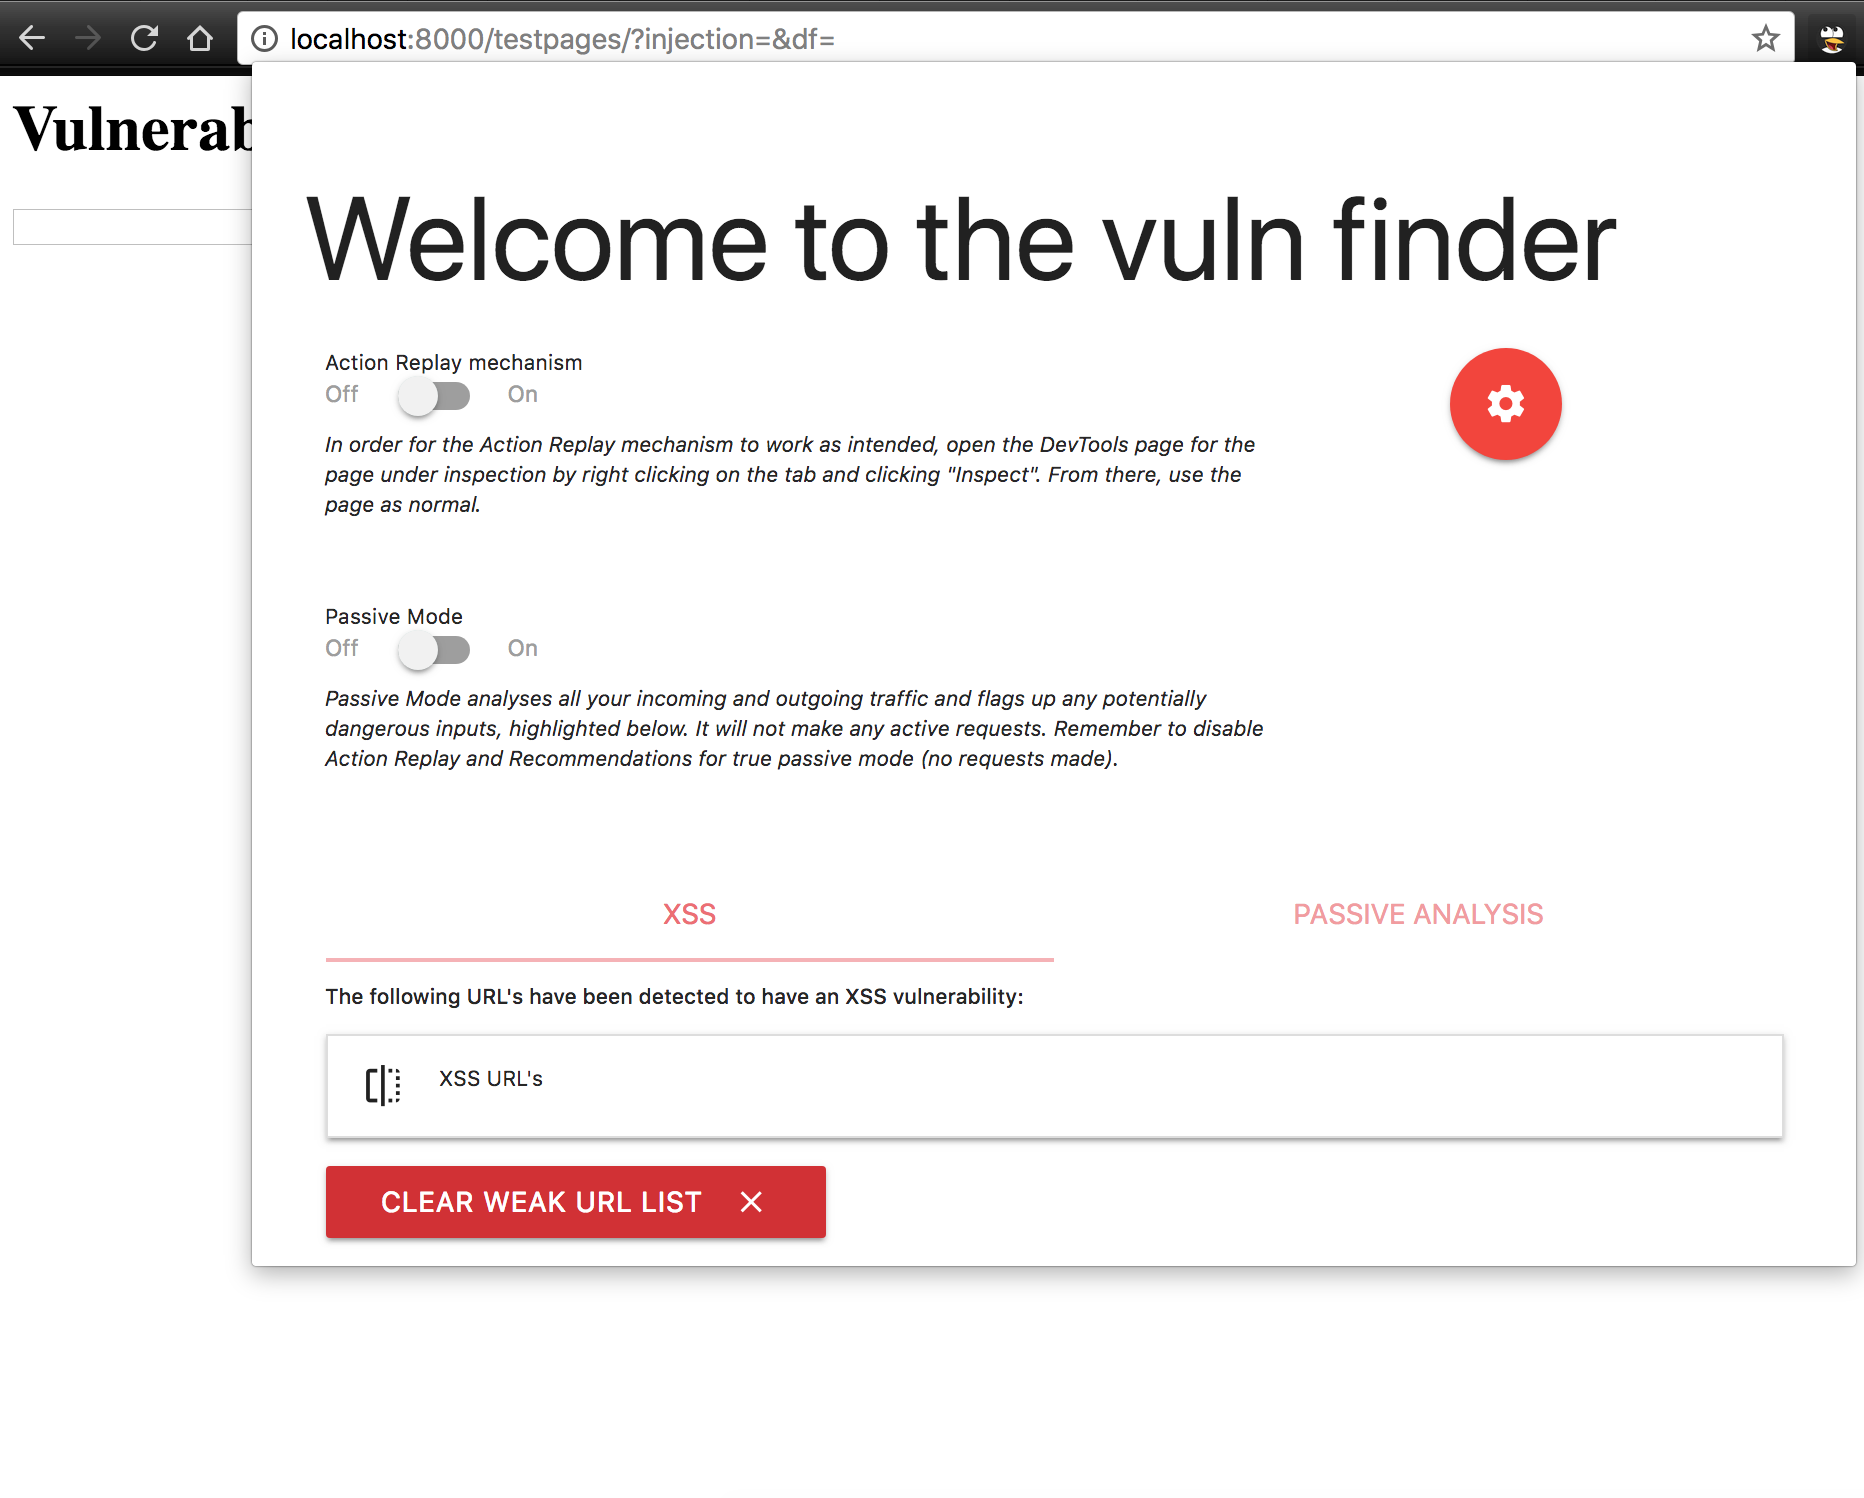
\includegraphics[width=0.8\textwidth]{images/first_look.png}
	\caption{The main contents of the popup page when first clicked by a user.}
	\label{fig:test}
\end{figure}

\begin{figure}[h]
	\centering
	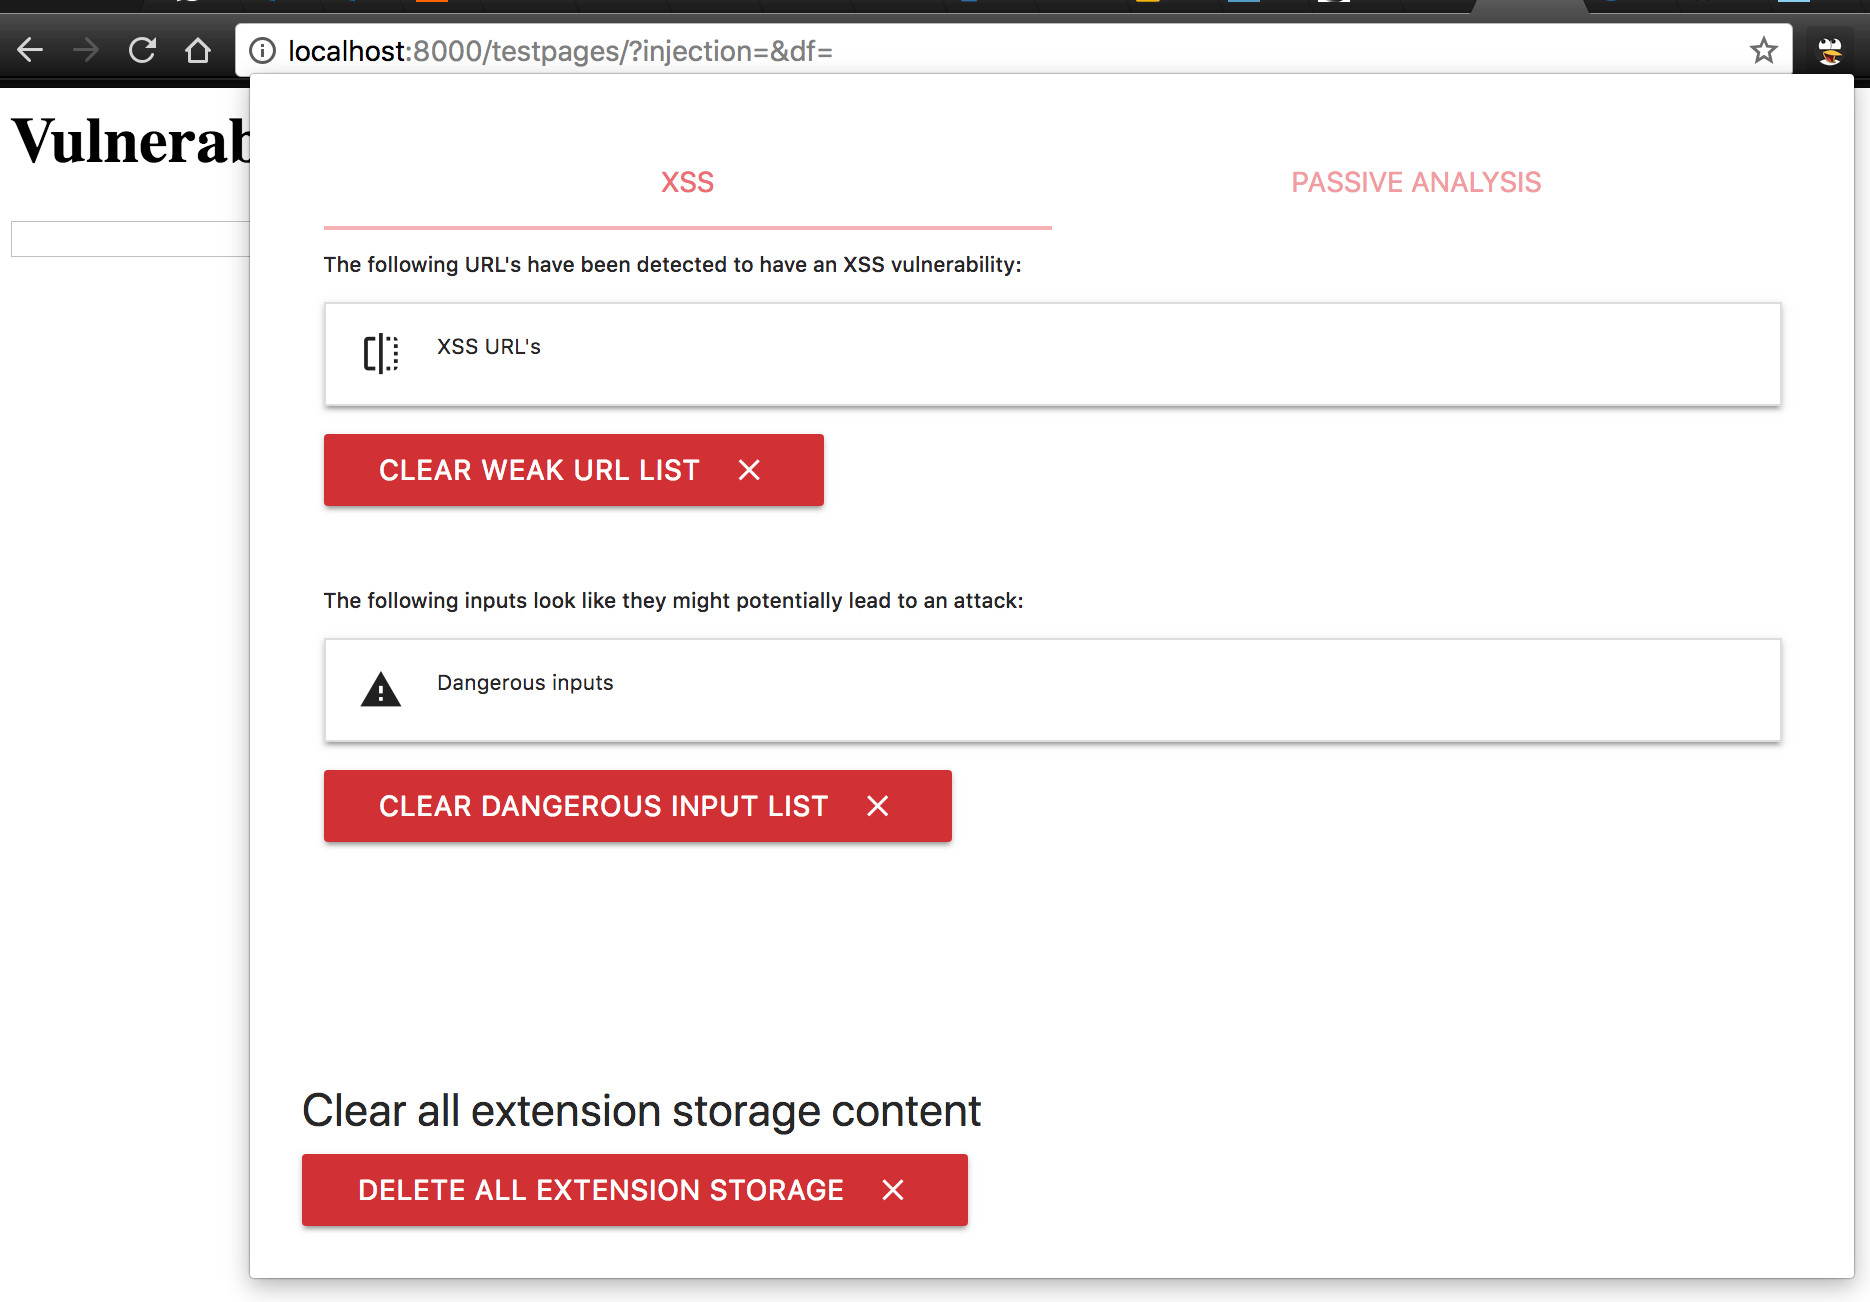
\includegraphics[width=0.8\textwidth]{images/popup_2.png}
	\caption{The main contents of the popup page when first clicked by a userw}
	\label{fig:test}
\end{figure}

This page offers an accessible means for tweaking and toggling all the options available in the extension, as well as viewing and analysing the outputs from the different modes of running the extension.  


\section{Background Page}

The background page I am using in the extension is a persistent page, meaning it is constantly running. This is in contrast to event background pages, which are opened and closed as necessary depending on the occasion. I am using this page to listen for messages sent from other scripts to be able to set aesthetic updates, as well as establishing a connection with the \texttt{devtools} page to subscribe to and forward custom request messages to content scripts.

\section{Message Design}



\section{Action Replay}



\section{Passive Mode}

Mention about 2 different ways of doing it - passive mode with normal cross checks by default - sliding window with eviction of requests.
Instead I keep window size and cross check only when enabled.

\subsection{Recommendations}